\documentclass{beamer}

\usepackage{tikz}
\usepackage{listings}
\usetikzlibrary{automata,positioning}
\usepackage{attrib}
\usepackage{color}
\usepackage{url}
\usepackage{todo}
\usepackage{fancyvrb}

\usetikzlibrary{er}
\title{Verifying Type Class Laws with Equational Reasoning}
\subtitle{A description by example}
\author{Lukas Hofmaier \texttt{lukas.hofmaier@hsr.ch}}
\date{June 12, 2015 \\ Progam Analysis and Transformation Seminar FS15}

\begin{document}
\maketitle
\begin{frame}
  \frametitle{Outline}
  \tableofcontents
\end{frame}

\section{Motivation}

\begin{frame}
  \frametitle{Why I'm interested in the topic?}
 An often touted property of pure functional languages is referential transparency.
\begin{figure}
  \centering
     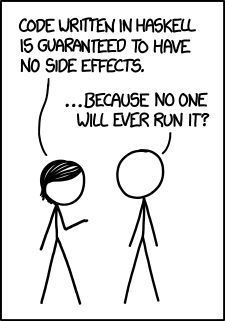
\includegraphics[width=0.3\textwidth]{sideeffects}
\end{figure}

\end{frame}

\begin{frame}[fragile]
\frametitle{What is referential transparency?}
Computation yields the same value each time it is invoked
\begin{Verbatim}[commandchars=\\\{\}]
y =  f x
g = h \textcolor{red}{y y} 
\end{Verbatim}
We can replace the definition of \verb|g| with
\begin{Verbatim}[commandchars=\\\{\}]
g = h \textcolor{red}{(f x) (f x)}
\end{Verbatim}
and get the same result.

\end{frame}
\section{Equational Reasoning}
\subsection{Referential Transparency}
\subsection{Reasoning about algebraic properties}

\begin{frame}
  \frametitle{What is equational reasoning?}

Equational reasoning is a method originally used in algebra.
 It's the process of proving a given property by substituting equal expressions. 
\begin{equation*}
  \label{eq:sum}
  (x+a)(x+b) = x^2 + (a+b)x+ab
\end{equation*}
\pause
\begin{equation*}
  (x+a)(x+b) = x^2 + ax + xb + ab \text{     (use distributivity)}
\end{equation*}
\pause
\begin{equation*}
x^2 + ax + {\color{red} xb} + ab = x^2 + ax + {\color{red} bx} + ab \text{     (use commutativity)}
\end{equation*}
\pause
\begin{equation*}
x^2 + {\color{red} ax + bx} + ab = x^2 + {\color{red}(a + b)x} + ab \text{     (use distributivity)}
\end{equation*}
 \footnotetext{Example taken from Graham Hutton, Programming in Haskell}
\end{frame}

\subsection{Reasoning about programs}

\begin{frame}[fragile]
  \frametitle{Reasoning about programs}
  We can reason the same way about programs.

For instance, we want to verify the following property.
\begin{verbatim}
length [x] = 1
\end{verbatim}
Given the function definition of \verb|length|.
\begin{verbatim}
length [] = 0
length (x:xs) = 1 + length xs  
\end{verbatim}
\end{frame}

\begin{frame}[fragile]
  \frametitle{Reasoning about programs}
  \begin{block}{Definitions}
    \begin{verbatim}
length [] = 0
length (x:xs) = 1 + length xs  
\end{verbatim}
  \end{block}
  \begin{block}{Step-by-step substitution}
    

Begin from the left-hand side \verb|length [x]| and try to get to the right-hand side \verb|1| by substituting equals-for-equals.

\begin{Verbatim}[commandchars=\\\{\}]
length \textcolor{red}{[x]}         -- [x] is the same as x:[]
\end{Verbatim}
\pause
\begin{verbatim}
= length (x:[])    -- apply definition
\end{verbatim}
\pause
\begin{Verbatim}[commandchars=\\\{\}]
= 1 + \textcolor{red}{length []}    -- apply definition
\end{Verbatim}
\pause
\begin{verbatim}
= 1 + 0            --  1 + 0 = 1
= 1
\end{verbatim}
  \end{block}
\end{frame}

\section{Type Classes}

\begin{frame}[fragile]
\frametitle{Type Classes}
  \begin{block}{Type classes}
    \begin{itemize}
   \item Describes the behavior of a type.
    \item  Type class is a construct that supports overloaded functions and ad hoc polymorphism
  \item An overloaded function uses different function definitions depending on the types of the arguments
  \item constrains the type variable in the type signature declaration \verb|t|. \verb|t| has to be a member of \verb|Show|.
  \end{itemize}
\end{block}
\begin{block}{Example}
\begin{Verbatim}
showlist :: Show t => [t] -> String
showlist [] = ""
showlist (x:xs) = show x ++ showlist xs
\end{Verbatim}

\end{block}
\end{frame}

\begin{frame}
\frametitle{Relation of type classes, types and values}

  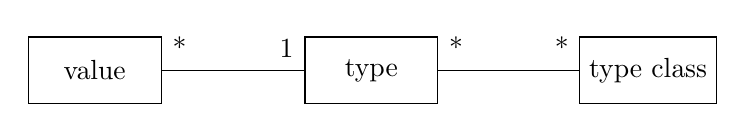
\begin{tikzpicture}[node distance=10em]
  \node[entity](type){type};
  \node[entity](typeclass)[right of=type]{type class};
  \node[entity](value)[left of=type]{value};
  \draw (type) -- (typeclass) node [very near end, above=1pt] {*} node [very near start, above=1pt] {*};
\draw (value) -- (type) node [very near end, above=1pt] {1} node [very near start, above=1pt] {*};
\end{tikzpicture}    

\end{frame}

\begin{frame}[fragile]
\frametitle{Type class laws}
\begin{block}{Laws}
\begin{itemize}
\item Type classes exhibit type class laws
\item Laws ensures expected behavior (e.g. associativity)
\item The Haskell compiler does not enforce type class laws.
\item We can use laws to apply equational reasoning
\end{itemize}  
\end{block}

\begin{block}{Example}
The left identity law states that \verb|mempty| has to behave like the identity element with respect to \verb|mappend|.
\begin{Verbatim}[fontsize=\small]
mappend mempty x = x
\end{Verbatim}  
\end{block}
\end{frame}

\begin{frame}
\frametitle{Relation of type classes with equational reasoning}
  \begin{figure}
  \centering
     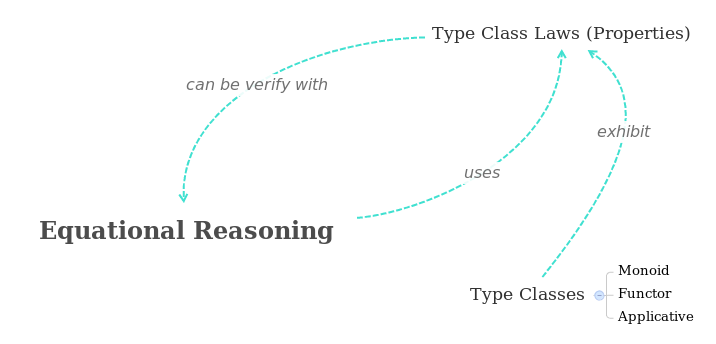
\includegraphics[scale=0.4]{mindmap}
\end{figure}
\end{frame}

\lstset{
basicstyle=\ttfamily,
columns=fullflexible,
keepspaces=true,
captionpos=b
}

\section{Example Proof for a Monoid Law }

\begin{frame}[fragile]
\frametitle{Example Proof for a Monoid Law}
  Suppose we want to build a plugin system

  \begin{block}{Plugin}
A plugin in our example is an \verb|IO| action that takes a \verb|Char| value and does some work with it (e.g. log to a file) It has type \verb|Char -> IO ()|.\end{block}

\begin{block}{Usage}
\begin{verbatim}
main = do
    c <- getChar
    logto c
\end{verbatim}
\end{block}
\end{frame}

\begin{frame}[fragile]
\frametitle{Requirements}
\begin{block}{Composability}
\begin{Verbatim}[fontsize=\footnotesize]
composedPlugin :: Char -> IO ()
composedPlugin  = logto `mappend` print2stdout
\end{Verbatim}

\begin{Verbatim}[fontsize=\footnotesize]
-- mappend :: Plugin -> Plugin -> Plugin
\end{Verbatim}

Both arguments are of type \verb|Char -> IO ()|. The return value is also of type \verb|Char -> IO ()|.
\end{block}
\begin{block}{Associativity}
The order of evaluation must not matter.
\begin{Verbatim}[fontsize=\footnotesize]
composed1 = logto `mappend` (print2stdout `mappend` donothing)
composed2 = (logto `mappend` print2stdout) `mappend` donothing
\end{Verbatim}
  
\end{block}
\end{frame}

\begin{frame}[fragile]
  \frametitle{Monoids to the rescue}

There is a type class for this behavior.

\begin{itemize}
\item A monoid is when you have an associative binary function and a value which acts as an identity. Types which behave like monoids can be part of the type class \verb|Monoid|. For example list \verb|[]| under concatenation is a \verb|Monoid|.
\item The monoid laws state that \verb|mappend| must be associative.
\item If \verb|mappend| satisfies the monoid laws then we are able to add plugins without concerning about the order of evaluation.
\end{itemize}

\end{frame}

\begin{frame}[fragile]
\frametitle{Example Proof for a Monoid Law}  
\begin{block}{Instance implementation}
Members of the type class \verb|Monoid| have to implement the functions \verb|mempty| and \verb|mappend|.
  \begin{Verbatim}[fontsize=\footnotesize]
    instance (Applicative f, Monoid a) => Monoid (f a) where
        mempty = pure mempty
        mappend = liftA2 mappend
  \end{Verbatim}
\end{block}
\begin{block}{Left identity law}
The left identity law states that \verb|mempty| has to behave like the identity element with respect to \verb|mappend|.
\begin{Verbatim}[fontsize=\footnotesize]
mappend mempty x = x
\end{Verbatim}  
\end{block}

\end{frame}

\begin{frame}[fragile]
  \frametitle{Proof of the monoid laws}
 \let\thefootnote\relax\footnotetext{Example from www.haskellforall.com}
\begin{verbatim}
mappend mempty x                 -- apply def. mappend
\end{verbatim}
\pause
\begin{verbatim}
= liftA2 mappend mempty x        -- apply def. mempty
\end{verbatim}
\pause
\begin{verbatim}
= liftA2 mappend (pure mempty) x -- apply def. of liftA2
\end{verbatim}
\pause
\begin{verbatim}
= (pure mappend <*> pure mempty) <*> x   
\end{verbatim}

\end{frame}


\begin{frame}[fragile]
  \frametitle{Proof of the monoid laws}
\verb|Applicative| type class instances satisfy the following laws:
\begin{itemize}
\item
\begin{Verbatim}
pure f <*> pure x = pure (f x)
\end{Verbatim}
\item
\begin{Verbatim}
pure id <*> x = x
\end{Verbatim}
\end{itemize}

We can use this property to substitute the left-hand side.
\begin{Verbatim}[commandchars=\\\{\}]
\textcolor{red}{(pure mappend <*> pure mempty)} <*> x   
\end{Verbatim}
\pause
\begin{Verbatim}[commandchars=\\\{\}]
= pure (\textcolor{red}{mappend mempty}) <*> x  -- transform to lambda
\end{Verbatim}
\pause
\begin{Verbatim}[commandchars=+\{\}]
= pure (\a -> +textcolor{red}{mappend mempty a}) <*> x -- 1. monoid law 
\end{Verbatim}
\pause
\begin{Verbatim}[commandchars=+\{\}]
= pure +textcolor{red}{(\a -> a)} <*> x                  -- a -> a = id
\end{Verbatim}
\pause
\begin{Verbatim}
= pure id <*> x                    -- applicative law
= x
\end{Verbatim}

\end{frame}

\begin{frame}
  \frametitle{Conclusion}
  \begin{itemize}
  \item Referential transparency makes it possible to conduct equational reasoning
\item The process of proving a property is cumbersome and difficult
\item Equational reasoning provides certainty that a program has particular properties. 
\end{itemize}

\end{frame}

\begin{frame}
  \frametitle{For Further Reading}

  \begin{thebibliography}{Subramaniam, 2011}

\bibitem{hutton}
Graham Hutton,
Programming in Haskell,
Cambridge University Press,
2007.

\bibitem{gonzales}
Gabriel Gonzales,
Equational reasoning at scale, 
\url{http://www.haskellforall.com}.

\end{thebibliography}
\end{frame}

\appendix

\subsection{Why use equational reasoning?}
\begin{frame}
\frametitle{Why use equational reasoning?}
\begin{block}{Example Property}
Correctness of a program can be specified in the form of an equation.
\begin{equation}
\text{fmap } \text{id}  =  \text{id}  
\end{equation}
We can use equational reasoning to verify if a property holds.  
\end{block}
\begin{block}{Goals of verification}
\begin{itemize}
\item Provide certainty that a program has particular properties
\item Contributes to the reliability and robustness of a software
\end{itemize}  
\end{block}
\begin{block}{Examples of use}
Example of use
\begin{itemize}
\item the first formally verified micro kernel, seL4.
\item streaming library "pipes"
\end{itemize}  
\end{block}
\end{frame}



\begin{frame}[fragile]
  \frametitle{Comparison of testing and proving properties}
  Suppose we want to check if the following equations holds
\begin{verbatim}
reverse reverse xs = xs
\end{verbatim}
How do we check that?
\begin{itemize}
\item Testing
\item Property-based testing
\item Proof that property holds
\end{itemize}

\end{frame}

\begin{frame}[fragile]
  \frametitle{Testing}
 In order to check the behavior, a function evaluates both sides of equation and compares the values
\begin{verbatim}
input = [1,2,3]
test_reverse :: Bool
test_reverse = reverse (reverse input) == input
\end{verbatim}
\end{frame}

\begin{frame}
  \frametitle{Comparison of testing and proving properties}
  \begin{description}
  \item[Testing] Code is compiled and executed. Can expose error. Cannot proof absence of errors. 
  \item[Proof] Properties hold under all circumstances.
\end{description}
\end{frame}

\begin{frame}
  \frametitle{Comparison of testing and proving properties}
\begin{figure}
  \centering
     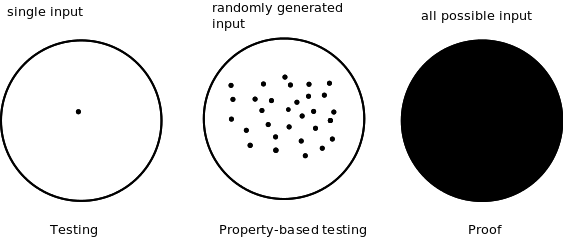
\includegraphics[width=1\textwidth]{testing}
\end{figure}
\end{frame}


\begin{frame}[fragile]
\frametitle{Proof by structural induction}
 \begin{description}
 \item[Base case] Prove $p(0)$ is true.
 \item[Induction step] Prove $p(n+1)$ if $p(n)$ (induction hypothesis) is true.
 \end{description}
\end{frame}

\begin{frame}[fragile]
\frametitle{Example proof by structural induction}
The length of two concatenated lists $xs$ and $ys$, is the same as the sum of the length of $xs$ and the length of $ys$
\begin{verbatim}
length (xs ++ ys) = length xs + length ys
\end{verbatim}

\end{frame}

\begin{frame}[fragile]
\frametitle{Base case}
We have to show that the property holds for the base case, the empty list \verb|[]|
\begin{verbatim}
length ([] ++ ys) = length [] + length ys
\end{verbatim}
\begin{columns}
  \begin{column}{.5\textwidth}
    \begin{block}{Left-hand side}
      \begin{verbatim}
length ([] ++ ys)
= length ys
\end{verbatim}
    \end{block}
  \end{column}
  \begin{column}{.5\textwidth}
    \begin{block}{Right-hand side}
\begin{verbatim}
length [] + length ys   
= 0 + length ys
= length ys
\end{verbatim}
    \end{block}
  \end{column}
\end{columns}
\end{frame}

\begin{frame}[fragile]
\frametitle{Induction step}
We have to show that if the equation holds for any list \verb|xs| then it also holds for \verb|x:xs|
\begin{verbatim}
pplength ([] ++ ys) = length [] + length ys
\end{verbatim}
\begin{columns}
  \begin{column}{.5\textwidth}
    \begin{block}{Left-hand side}
      \begin{verbatim}
length ((x:xs) ++ ys)      
= length (x:(xs ++ ys))    
= 1 + length (xs ++ ys)    
= 1 + length xs + length ys
\end{verbatim}
    \end{block}
  \end{column}
  \begin{column}{.5\textwidth}
    \begin{block}{Right-hand side}
\begin{verbatim}
length (x:xs) + length ys
1 + length xs + length ys
length [] + length ys   
\end{verbatim}
    \end{block}
  \end{column}
\end{columns}

\end{frame}


\begin{frame}[fragile]
  \frametitle{An Applicative can be a monoid}
\begin{figure}
  \centering
     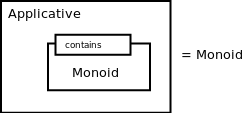
\includegraphics[width=0.7\textwidth]{monoid}
\end{figure}
\end{frame}


\begin{frame}[fragile]
\frametitle{Reusability of proof}
General implementation for \verb|mappend|. If \verb|f| is an \verb|Applicative| and \verb|b| is a \verb|Monoid| then \verb|f b| is also a \verb|Monoid|
\begin{verbatim}
{-# LANGUAGE FlexibleInstances #-}
{-# LANGUAGE OverlappingInstances #-}

instance (Applicative f, Monoid a) => Monoid (f a) where

  mempty = pure mempty
  mappend = liftA2 mappend
\end{verbatim}
\begin{itemize}
\item To prove a type class law we can use equational reasoning.
\item Type classes allow us to generalize definitions. A proof for the generalization is valid for all specializations.

\end{itemize}

\end{frame}

\begin{frame}[fragile]
\frametitle{Generalization of Proof}

\begin{enumerate}
\item The standard library provides a \verb|Monoid| instance for \verb|()| 

\item  \verb|IO ()| is a \verb|Monoid| because \verb|IO| is part of the \verb|Applicative| type class and \verb|()| is a \verb|Monoid|. The type \verb|(->) r| (that's the type of Haskell functions) is a part of the \verb|Applicative| type class.

\item 
\verb|Char -> IO ()| is a \verb|Monoid| because \verb|(->) Char| is an \verb|Applicative| and \verb|IO ()| is a \verb|Monoid|.

\end{enumerate} 
\end{frame}

\end{document}

%%% Local Variables: 
%%% mode: latex
%%% TeX-master: t
%%% End: 
